\usepackage{amsmath}
\usepackage{amssymb}
\usepackage{booktabs}
\usepackage{xcolor}
\usepackage{textcomp}
%\usepackage[caption=false,font=footnotesize]{subfig}
\usepackage[autostyle]{csquotes}
\usepackage{wrapfig}
\usepackage{url}
\usepackage{microtype}
\usepackage{lipsum}
\usepackage{adjustbox}
\usepackage{epstopdf}
%\usepackage[table]{xcolor}
%\usepackage{tabularx}
%\usepackage{listings}

\bibliographystyle{acmsiggraph-doi}

\newlength{\columnsepOriginal}
\setlength{\columnsepOriginal}{\columnsep}
\setlength{\intextsep}{0cm}

%% Bibliography hack
\makeatletter
\let\oldbibliography\thebibliography
\renewcommand{\thebibliography}[1]{%
  \oldbibliography{#1}%
  \setlength{\itemsep}{8pt}% % uncommment to tweak spaces
}
\makeatother

\title{Oil Paint Filtering using Color Palettes for Colorization}

\author{Amir Semmo \qquad \qquad J{\"u}rgen D{\"o}llner}

\institute{Hasso Plattner Institute, Germany}

\pdfauthor{Amir Semmo}

\begin{document}

\maketitle

\begin{columns}

	\column{0.25}
	
	\block{\blocktitle{}{Abstract}}{
	
		\setlength{\columnsep}{1cm}%
		\begin{wrapfigure}[7]{O}{0.25\linewidth}
			\begin{center}
				
\includegraphics[width=1.0\linewidth]{./resources/qrcode_abstract.eps}
			\end{center}
			\label{fig:qrcode_abstract}
		\end{wrapfigure}
	
		We present a novel technique for oil paint filtering that uses color palettes for colorization. First, dominant feature-aware colors are derived from the input image via entropy-based metrics. Seed pixels are then determined and propagated to the remaining pixels by adopting the optimization framework of Levin et al. \shortcite{Levin2004} for feature-aware colorization. Finally, the quantized output is combined with flow-based highlights and contour lines to simulate paint texture. Our technique leads to homogeneous outputs in the color domain and enables interactive control over color definitions.
	}
	
	\block{\blocktitle{1}{Introduction}}{
		\emph{Image-based artistic rendering} received significant attention in the past decades, covering a broad range of expressive rendering styles for visual communication \cite{Kyprianidis2013}.
		Most approaches are based on edge-preserving filtering to reduce image details without loss of salient structures, e.g., by locally weight averaging in the color domain and range, or by solving an optimization problem for image decomposition.
		However, these approaches are typically limited in not being able to process image contents according to a pre-defined color palette, which is often a desired feature by artists to have creative control over the filtered output.
		To this end, we present an inverse filtering approach that derives dominant color tones from an input image and uses them for feature-aware colorization, which we demonstrate by a novel oil paint effect. We base our technique on the optimization framework of Levin et al. \shortcite{Levin2004} to simulate the way artists paint with a reduced color palette, and combine the results with the flow-based computations by Kyprianidis and D{\"o}llner \shortcite{Kyprianidis2008} to simulate paint texture.
		Our technique produces more homogeneous color distributions than local filtering, and gives artists more control in refining basic color tones used for visualization.
	}
	
	\block{\blocktitle{2}{Implementation}}{
		The $600 \times 812$ pixel image shown in Figure \ref{fig:result_1} was processed on an Intel\textregistered~Xeon\texttrademark~4 $\times$ 3.06 GHz and NVidia\textregistered~GTX 760 GPU in 52 seconds. Both the flow computation and DoG filtering perform in real time for images with HD resolution.
		The major strength of our technique is that it allows users to easily redefine color tones. We plan to build on this functionality for user-defined color theme adjustment \cite{Wang2010}.
		Further, we plan to improve the flow visualization by using a distance transform on the contour lines of the colorized output, i.e., to synthesize flow lines that better follow feature contours in areas of constant color tones.
		Because the flow computation performs in real-time, it may also be interactively refined via a painting interface.
	}
	
	\column{0.5}
	
	\block{\blocktitle{3}{Method}}{
		\begin{tikzfigure}[Schematic overview of our technique that automatically transforms color images~(left) to filtered variants with oil paint characteristics~(right). First, a color palette is derived from the input image (here: 25 distinct color tones) and is used as input for colorization. The quantized image is then combined with a thresholded flow field to simulate oil paint, together with a difference-of-Gaussians filtering to include contour lines. (Original photograph from flickr.com and kindly provided under Creative Commons license by Tomas Sobek.)]
			\centering
			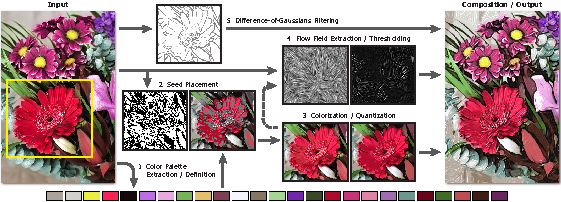
\includegraphics[width=1.0\linewidth]{./resources_poster/teaser.pdf}
  			\label{fig:teaser}
		\end{tikzfigure}
	}
	
	\block{\blocktitle{4}{Overview}}{
    	\begin{minipage}[t]{1.0\linewidth}
    	\begin{multicols*}{2}
      An overview of our approach is shown in Figure \ref{fig:teaser}. It performs in a series of four major stages:\\
      
    	\begin{enumerate}
			\item \textbf{Feature-aware Extraction of Color Palettes} -- We seek to derive colors in local image regions for a feature-aware color extraction.
We implemented a scoring system to iteratively determine image regions of constant color tones. The scores are based on weighted entropy values, luminance to prefer vivid colors, and difference to previously derived colors to prefer a broad color spectrum.\\
			\item \textbf{Placement of Color Seeds} -- The color difference ($\Delta E^*$) between each pixel of the input image and entry of the derived color palette is computed. If the difference falls below a given threshold, the pixel is marked as seed and colored by the entry of the palette with the minimal difference. The seed pixels are used as \enquote{scribbles} for the colorization stage.\\
			\item \textbf{Colorization using Optimization} -- The input image is converted to CIE-Lab color space and used with the seed pixels to parameterize the colorization technique of Levin et al. \shortcite{Levin2004}. The technique propagates the color components to the remaining pixels by solving an optimization problem, i.e.,~pixels with similar intensities have similar colors. Afterwards, the luminance channel is filtered in a second pass: first the colorized output is converted to HSV color space, and then the \emph{hue} values are used to propagate the luminance values of the input image with the same seed pixels of the first pass. The filtered luminance values are then combined with the color values of the first pass to yield a quantized color image.\\
			\item \textbf{Flow-based Highlights and Contour Lines} -- The flow fields of the colorized output and input images are derived from the smoothed structure tensor according to the approach of Kyprianidis and D{\"o}llner \shortcite{Kyprianidis2008}. The magnitude of the visualized flow field is thresholded to yield a paint texture \cite{Hertzmann2002}. Optional difference-of-Gaussians (DoG) filtering~\cite{Gooch2004} is performed on the input image to include contour lines in the final image.\\
		\end{enumerate}

		All stages can be parameterized to enable artistic control over the filtering process: the total number of colors extracted and used as input for colorization, brush size and scale for the thresholded flow field, and scale of the contour lines. Figure \ref{fig:result_1} shows a comparison of our approach with the oil paint filter of Adobe Photoshop CS5. Notice how our approach is able to preserve feature contours and details while using a strong color quantization.

		We have implemented our filtering technique using C++ and CUDA. The color extraction is implemented on the CPU, and the remaining stages on the GPU.
		%
		%The $600 \times 812$ pixel image shown in Figure \ref{fig:result_1} was processed on an Intel\textregistered~Xeon\texttrademark~$4\times$ 3.06 GHz and NVidia\textregistered~GTX 760 GPU in 52 seconds. Both the flow computation and DoG filtering perform in real time for images with HD resolution.

		%The major strength of our technique is that it allows users to easily redefine color tones. We plan to build on this functionality for user-defined color theme adjustment \cite{Wang2010}.
		%
		%Further, we plan to improve the flow visualization by using a distance transform on the contour lines of the colorized output, i.e., to synthesize flow lines that better follow feature contours in areas of constant color tones.
		%
		%Because the flow computation performs in real-time, it may also be interactively refined via a painting interface.
	\end{multicols*}
	\end{minipage}%
      
	}
	
	\column{0.25}
	
	\block{\blocktitle{5}{Results}}{
		\begin{tikzfigure}[An image filtered with our technique using 24 distinct color tones. Our derived color palette is shown below. (Original photograph from flickr.com and kindly provided under Creative Commons license by Ludovic Hirlimann.)]
			\centering
			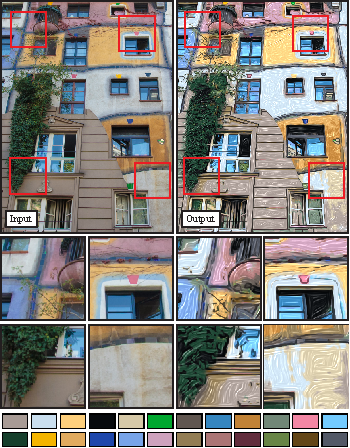
\includegraphics[width=1.0\linewidth]{./resources_poster/result_1.pdf}
  			\label{fig:result_1}
  		\end{tikzfigure}
	}
	
	\block{\blocktitle{}{References}}{
		\bibliography{bibliography}
	}
	
\end{columns}

\printfooter

\block{}{
	\begin{minipage}{7.72cm}
		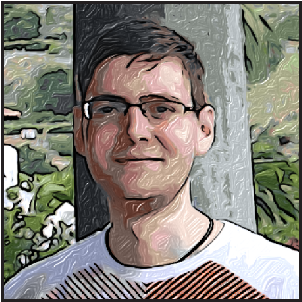
\includegraphics[width=\textwidth]{./resources/portrait.pdf}
	\end{minipage}
	\hspace{1.0cm}
	\begin{minipage}{16.05cm}
		\large\sffamily
		Amir Semmo, M.Sc.\\
		amir.semmo@hpi.de\\
		+49(0)331 5509 3909\\
		
		Computer Graphics Systems Group\\
		Hasso Plattner Institute\\
		www.hpi3d.de
	\end{minipage}
	\begin{minipage}{13.08cm}
		\large\sffamily
		Prof. Dr. J{\"u}rgen D{\"o}llner\\
		office-doellner@hpi.de\\
		~\\
		
		Hasso Plattner Institute\\
		Prof.-Dr.-Helmert-Str. 2--3\\
		D-14482 Potsdam, Germany
	\end{minipage}
	\begin{minipage}{7.13cm}
		\vspace{-0.5cm}
		\includegraphics[width=\textwidth]{./resources/qrcode_hpi3d.eps}
		\vspace{-1.6cm}
		\begin{center}
			\emph{www.hpi3d.de}
		\end{center}
	\end{minipage}
	\hfill
	\begin{minipage}{11.89cm}
		\begin{flushright}
			
\includegraphics[height=6cm]{./resources/hpi_logo_cmyk_wb_sl1.pdf}
		\end{flushright}
	\end{minipage}
	\begin{minipage}{11.3cm}
		\begin{flushright}
			\includegraphics[height=4cm]{./resources/4DnD-Logo.pdf}
		\end{flushright}
	\end{minipage}
	\begin{minipage}{13.67cm}
		\begin{flushright}
			\includegraphics[height=3cm]{./resources/inno-profile.png}
		\end{flushright}
	\end{minipage}
	\begin{minipage}{9.51cm}
		\begin{flushright}
			\includegraphics[height=5cm]{./resources/Logo-BMBF-EN.png}
		\end{flushright}
	\end{minipage}
}

\end{document}
